\section{The LZ Outer Detector} \label{OD_info}

\par
LZ uses linear akylbenze (LAB) - the generic term for this class of chemical compositions - as the liquid scintillator.
In this, neutron capture happens on the hydrogen; $n + p \xrightarrow{} d + \gamma$ with a capture constant of 200$\mu$s \cite{LZ_TechnicalDesignReview_ref}.
The hydrogen capture produces a single 2.2MeV $\gamma$.
\par
The scintillator in the OD is doped with 0.1\% (by mass) by Gadolinium.
This provides 

\begin{enumerate}
    \item cross section 49kb: (61kb for $Gd^{155}$ and 254kb for $Gd^{157}$)
    \item capture energy release: 8536.39keV ($Gd^{155} \xrightarrow{} Gd^{156}$) and 7937.39keV ($Gd^{157} \xrightarrow{} Gd^{158}$)
    \item More released particles (4.7, $\gamma$'s and $e^{-}$)
    \item neutron-capture time = 30$\mu$s
    \item 9000 optical photons per MeV. Not sure where this number has some from
\end{enumerate}

\par
LZ dopes with 0.1\% by mass (0.23 - 0.34\% by number)

\par
In addition to the gadolinium doping, the scintillator is also made up of two wavelength shifters; a primary shifter (or fluor) and a second wavelength shifter.
The fluor is 2,5-diphenyloxazole (PPO); an organic scintillator which converts shorter wavelength light to longer wavelength light. 
This has a spectrum peak at 385nm (UV).
The second wavelength shifter is 1,4-bis(2-methylstyryl(benzene)) (Bis-MSB). 
Bis-MSB absorbs the PPO scintillation and emits with peak of around 410-425nm.
The reason for the second shifter is that the wavelength emitted is absorbed less by the LS and is closer to the PMT response.
Importantly, the absorption length of the GdLS increases from 1m to in excess of 10m in that range - and continues to rise.

\par
The complete chemical components in the GdLS is shown in Table \ref{tab:GdLS_Components}.

\begin{table}[!htbp]
    \centering
    \begin{tabular}{c | c | c | c}
    \hline
    {Component (referred as)} & {Purpose} & {Weight (g/mol)} & {Mass (g)} \\ \hline
    $C_{17.14}H_{28.28}$ (LAB) & n,g & 234.4  & 853.55 \\
    $C_{15}H_{11}NO$ (PPO) & primary wavelength shifter & 221.3 & 3.00 \\
    $C_{24}H_{22}$ (Bis-MSB) & wavelength shifter & 310.4 & 0.015 \\
    $C_{9}H_{17}O^{-}_{2}$ (TMHA) & chelation agent & 157.2 & 2.58 \\
    natural gadolinium (Gd) & neutron capture & 157.3 & 0.86 
    \end{tabular}
    \caption{GdLS Components in 1L of GdLS}
    \label{tab:GdLS_Components}
\end{table} 

\par
Table \ref{tab:Gadolinium_abundances_and_crosssections} contains the natural abundances of gadolinium.

\begin{table}[!htbp]
    \centering
    \begin{tabular}{c | c | c}
    \hline
    {Isotope} & {Abundance (\%)} & {Cross-section (b)} \\ \hline
    $Gd^{152}$ & 0.2 & 735 \\
    $Gd^{154}$ & 2.18 & 85 \\
    $Gd^{155}$ & 14.80 & 60900 \\
    $Gd^{156}$ & 20.47 & 1.8 \\
    $Gd^{157}$ & 15.65 & 254000 \\
    $Gd^{158}$ & 24.84 & 2.2 \\
    $Gd^{160}$ & 21.86 & 1.4

    \end{tabular}
    \caption{Gadolinium natural abundances and thermal neutron capture cross-sections \cite{Gadolinium_abundances_and_crosssection_ref}}
    \label{tab:Gadolinium_abundances_and_crosssections}
\end{table} 

\paragraph{Other Properties}
It is also worth noting that proton scatters and $\alpha$'s have quenched scintillation signals.
For the proton, it is most easily described by the effect of neutron collisions.

\par
In the lab-frame, the ratio between a neutrons initial energy ($E$) and final energy ($E'$) when colliding with an at rest nucleus of mass A follows;
\begin{equation}
    \frac{E'}{E} = \frac{A^2 + 1 + 2A\cos{\theta}}{(A + 1)^2}
\end{equation}
where $\theta$ is the scattering angle in the CoM.
Now, if the nucleus is a hard sphere, so independent of $\theta$, then an elastic scatter follows
\begin{equation}
    E^{'} = E(\frac{A-1}{1})^{2}
\end{equation}
If A = 1 (so is a proton), then it reduces further to $E^{'} = \frac{1}{2}E$, meaning that the neutron loses half its energy on average.
The scattered proton has energy $E - E^{'}$ and is quenched.



\subsection{Neutrons in GdLS}

\subsubsection{background neutrons}
\par
Maybe this and DD neutrons into a separate section before GdLS section?

\subsubsection{DD neutrons}
\par
10,000 DD simulations have been done - a mono-energetic neutron source which LZ will be using for calibration purposes.
Neutrons are emitted at 2.45MeV.

\par
From these simulations (performed on BACCARAT release 6.2.1).
Table \ref{tab:Where_neutrons_go} shows the number neutrons which enter the scintillator and have their final stage there.
The vast majority of the neutrons emitted enter and are captured in the parts of the detector immediately surrounding where it originated.
Importantly, only 23\% of neutrons which remain in the detector finish in the scintillator.
This could be Gd-capture, H-capture, or something else.

\begin{table}[!htbp]
    \centering
    \begin{tabular}{c | c | c  }
    \hline
    {Final Volume}  & {Where all go (\%)} & {Where all go - ignoring OutOfWorld (\%)} \\ \hline
    WaterAndPMTs & 33.59 & 42.55 \\
    OutOfWorld & 21.06 & - \ \\
    ScintillatorCenter & 18.75 & 23.75 \\
    PVCNeutronTube & 15.06 & 19.08 \\
    LiquidXenonTarget & 2.39 & 3.03 \\
    ScintillatorTank & 2.16 & 2.74 \\
    OuterTitaniumVessel & 1.93 & 2.44 \\
    LiquidSkinXenon & 1.27 & 1.61 \\
    InnerTitaniumVessel & 1.19 & 1.51 \\
    WaterTank & 1.12 & 1.42 \\
    SteelNeutronTubeCaps & 0.8 & 1.01 \\
    Other & 0.68 & 0.86 
    \end{tabular}
    \caption{The volume within the detector where DD neutrons have their final step. OutOfWorld indicates that the neutron left the detector area and so the simulation stopped as it's path is not relevant. Other refers to any other part of the detector.}
    \label{tab:Where_neutrons_go}
\end{table} 

\par
Focusing on the neutrons which finish in the scintillator volume, we can in Table \ref{tab:Where_gdls_neutrons_go} that 78\% of neutrons which enter the GdLS end there.
However, it is also interesting to note that 702 neutrons (37\%) enter the scintillator, then leave the scintillator, then enter again (and then die there).

\begin{table}[!htbp]
    \centering
    \begin{tabular}{c | c | c | c }
    \hline
    {Neutron Description}  & {Raw Number} & {Percentage (\%)} & {Percentage remaining in detector (\%)} \\ \hline
    Enters GdLS            &     2406     & 24.06                           & 30.4788 \\
    Dies in GdLS           &     1875     & 18.75                           & 23.7522 \\
    Enters and Dies        &     1875     & 77.9302                         & 77.9302
    
    \end{tabular}
    \caption{What happens to neutrons which enter the scintillator volume.}
    \label{tab:Where_gdls_neutrons_go}
\end{table} 

\par
Figure \ref{fig:dd_neutron_gdls_kinetic_energy_vs_number_of_interactions} shows that on average a neutron will have 27 interactions in the scintillator (excluding transportation steps).

%\pgfplotsset{
%  /pgfplots/colormap={coldredux}{
%    [1cm]
%    rgb255(0cm)=(255,255,255)
%    rgb255(1cm)=(0,192,255)
%    rgb255(3cm)=(0,0,255)
%    rgb255(6cm)=(0,0,0)
%  }
%}

\begin{figure}[!htbp]%
\centering
\begin{tikzpicture}
\centering
  \begin{axis}[%point meta max=150,
    %point meta min=0.0,
    view={0}{90},
    ylabel={Kinetic Energy (MeV)},
    xlabel={Number of Interactions},
    colorbar,
    colorbar style={ylabel={Count}},
    ]
    \addplot3[
      surf,
      shader=flat corner,
      mesh/cols=51,
      mesh/ordering=rowwise,
      point meta = {z<1 ? nan : z}
    ] file {Data/GdLS_Physics/Pre_Capture/dd_neutrons_gdls_initial_keV_vs_n_interactions.txt};
\end{axis}
\end{tikzpicture}
\caption{The relationship between the number of interactions a neutron has in the scintillator and the neutrons kinetic energy when it enters the liquid scintillator volume for neutrons which are 'captured' in the scintillator volume.
}
\label{fig:dd_neutron_gdls_kinetic_energy_vs_number_of_interactions}
\end{figure}


\begin{figure}[!htbp]%
\centering
\begin{tikzpicture}
\centering
  \begin{axis}[%point meta max=150,
    %point meta min=0.0,
    view={0}{90},
    ylabel={Distance before capture (mm)},
    xlabel={Number of Interactions},
    colorbar,
    colorbar style={ylabel={Count}},]
    \addplot3[
      surf,
      shader=flat corner,
      mesh/cols=119,
      mesh/ordering=rowwise,
      point meta = {z<1 ? nan : z}
    ] file {Data/GdLS_Physics/Pre_Capture/dd_neutrons_gdls_distance_travelled_vs_n_interactions.txt};
\end{axis}
\end{tikzpicture}
\caption{The relationship between the number of interactions a neutron has in the scintillator and the neutrons kinetic energy when it enters the liquid scintillator volume for neutrons which are 'captured' in the scintillator volume.
}
\label{fig:dd_neutron_gdls_distance_vs_number_of_interactions}
\end{figure}



\par
Plots to do:

\begin{itemize}
    \item time before capture
    \item captured on what (hydrogen or Gd)
    \item time vs kinE
    \item distance vs kinE
    \item fraction captured by Gd vs H
\end{itemize}


\subsection{Gd Neutron Capture}
\par
After the neutron capture the gadolinium enters an excited state. 
For $Gd^{156}$ this is 8536.39keV and for $Gd^{158}$ is 7937.39keV.
This energy is released as follows;

\begin{enumerate}
    \item Via gamma-rays emission from the decay of an excited nucleus
    \item Internal conversion which leads to
    \begin{enumerate}
        \item auger electron emission
        \item characteristic x-ray emission
    \end{enumerate}
\end{enumerate}


\subsubsection{Dicebox Simulations}
\par
Geant4 is unable so accurately simulate accurately some $\gamma$-decay from excited nuclei.
LUX-ZELPIN circumvented this by using DICEBOX - a monte-carlo package for simulating these decays.
Given that $Gd^{155}$ and $Gd^{157}$ have the largest cross sections and together account for 30\% of abundance, only those were simulated.
The results of these simulations are summarised in this section, and are selected randomly during LZ simulations.

\par
Figure \ref{fig:Gd_capture_resulting_particle_count} shows the number of discrete packets of energy over which the energy is released after the capture.
The mean value of this (from the 10 million simulations) is 4.654 and 4.754 for $Gd^{156}$ and $Gd^{158}$ respectively.
This is why it is often quoted that the neutron capture releases 4.7 $\gamma$'s.

\begin{figure}[!htbp]
    \centering
    \begin{tikzpicture}
        \begin{axis}[title=N. de-excitation energy transition steps from Gadolinium neutron captures,
            xlabel=N. Steps,
            ylabel=,
            width=15cm,
            height=6cm,
            xmin=0,
            xmax=13,
            ymin=0,
            legend pos=north east,]
            \addplot[red, const plot]
                    table [x=Lower,y=Weight]
                    {Data/GdLS_Physics/DICEBOX/gd156_n_steps.txt};
                \addlegendentry{$Gd^{156}$};
            \addplot[blue, const plot]
                    table [x=Lower,y=Weight]
                    {Data/GdLS_Physics/DICEBOX/gd158_n_steps.txt};
                \addlegendentry{$Gd^{158}$};
        \end{axis}
    \end{tikzpicture}
    \caption{Result of 10 million DICEBOX simulations (5 million of both $Gd^{155}$ and $Gd^{157}$) showing in how many stages the energy is released from the atom.}
    \label{fig:Gd_capture_resulting_particle_count}
\end{figure}

\par
The simulation encompasses both $\gamma$-emission from the nucleus directly as well as the transfer of energy to an electron (internal conversion).
Where the energy goes within the atom is shown in Table \ref{tab:Gd_internal_energy_conversion}.
It shows that there is also a gamma emitted and that roughly 30\% of the time only $\gamma$'s are emitted, however it is most likely that energy is also passed to a shell electron.
From this, we can conclude that the dominant emission from the neutron capture are $\gamma$'s, with auger electrons and x-rays comprising a much smaller percentage of the emission.
\par
A less useful Figure is Figure \ref{fig:Gd_capture_energy_conversion_shells} shows where the energy goes in terms of electron shells. 

\begin{table}[!htbp]
    \centering
    \begin{tabular}{c | c | c | c | c | c | c}
    \hline
    {Excited Isotope}  & {$\gamma$-only} & {$\gamma$ + 1$e^{-}$} & {$\gamma$ + 2$e^{-}$} & {$\gamma$ + 3$e^{-}$} & {$\gamma$ + 4$e^{-}$+} & {$e^{-}$-only}\\ \hline
    $Gd^{156}$         & 29.8055         & 65.1064               & 5.00976               & 0.07648               & 0.00186               & 0.0        \\
    $Gd^{158}$         & 26.8031         & 67.0329               & 6.09488               & 0.06848               & 0.00064               & 0.0
     
    \end{tabular}
    \caption{Gadolinium nuclei de-excitation path by percentage. In this table, $e^{-}$ refer internal conversion, when the nucleus transfers energy to a shell electron.}
    \label{tab:Gd_internal_energy_conversion}
\end{table} 

\begin{figure}[!htbp]
    \centering
    \begin{tikzpicture}
        \begin{axis}[title=Fraction of steps going to internal conversion vs directly to $\gamma$'s,
            xlabel=Energy Transfer location,
            ylabel=Percentage of steps,
            width=15cm,
            height=6cm,
            legend pos=north east,
            xtick=data,
            xticklabels from table={Data/GdLS_Physics/DICEBOX/gd158_energy_conversion_to_shells.txt}{Label}]
            \addplot[red, const plot]
                    table [x=Bins, y=Weight]
                    {Data/GdLS_Physics/DICEBOX/gd158_energy_conversion_to_shells.txt};
                \addlegendentry{$Gd^{156}$};
            \addplot[blue, const plot]
                    table [x=Bins, y=Weight]
                    {Data/GdLS_Physics/DICEBOX/gd156_energy_conversion_to_shells.txt};
                \addlegendentry{$Gd^{158}$};
        \end{axis}
    \end{tikzpicture}
    \caption{DICEBOX simulation showing where the energy goes. On average each excited nucleus transfers it's energy in 4.7 steps, so the majority of the energy is transferred to $\gamma$'s. This figure isn't actually that helpful.}
    \label{fig:Gd_capture_energy_conversion_shells}
\end{figure}

\par
The proportion of the energy transferred directly to $\gamma$'s vs via internal conversion is shown in Figure \ref{fig:Gd_deexcitation_energy_fractions}.

\begin{figure}[!htbp]%
\centering
\begin{tikzpicture}
\centering
  \begin{groupplot}[view={0}{90},
    group style = {group size = 2 by 1}]
    \nextgroupplot[
    xmin=0,
    xmax=100,
    ymode=log,
    xlabel={Percentage of Energy (\%)},
    ylabel={Count},]
    \addplot[ybar interval, red, const plot]
            table [x=Lower,y=Weight]
            {Data/GdLS_Physics/DICEBOX/gd156_energy_fraction_gamma.txt};
    \addlegendentry{$Gd^{156}$-$\gamma$};
    \addplot[ybar interval, blue, const plot]
                    table [x=Lower,y=Weight]
                    {Data/GdLS_Physics/DICEBOX/gd156_energy_fraction_electron.txt};
    \addlegendentry{$Gd^{156}$-IC};
    \nextgroupplot[
    xmin=0,
    xmax=100,
    ymode=log,
    xlabel={Percentage of Energy (\%)}]
    \addplot[ybar interval, red, const plot]
            table [x=Lower,y=Weight]
            {Data/GdLS_Physics/DICEBOX/gd158_energy_fraction_gamma.txt};
    \addlegendentry{$Gd^{156}$-$\gamma$};
    \addplot[ybar interval, blue, const plot]
                    table [x=Lower,y=Weight]
                    {Data/GdLS_Physics/DICEBOX/gd158_energy_fraction_electron.txt};
    \addlegendentry{$Gd^{156}$-IC};
  \end{groupplot}
\end{tikzpicture}
\caption{The fraction of energy from the excited nucleus which goes to $\gamma$'s and to internval conversion.
\textbf{Left:} $Gd^{156}$ de-excitation path.
\textbf{Right:} $Gd^{158}$ de-excitation path.
}
\label{fig:Gd_deexcitation_energy_fractions}
\end{figure}




\par
Given what has been determined above, it is worth looking at the $\gamma$ spectrum, shown in Figure \ref{fig:Gd_capture_resulting_gamma_spectrum}.


\begin{figure}[!htbp]
    \centering
    \begin{tikzpicture}
        \begin{axis}[title=$\gamma$ energy spectrum from $Gd^{155}$ and $Gd^{157}$ neutron captures,
            xlabel=Energy (KeV),
            ylabel=,
            width=15cm,
            height=6cm,
            xmin=0,
            xmax=8000,
            ymin=0,
            legend pos=north east,]
            \addplot[red, const plot]
                    table [x=Lower,y=Weight]
                    {Data/GdLS_Physics/DICEBOX/gd156_gamma_spectrum.txt};
                \addlegendentry{$Gd^{156}$};
            \addplot[blue, const plot]
                    table [x=Lower,y=Weight]
                    {Data/GdLS_Physics/DICEBOX/gd158_gamma_spectrum.txt};
                \addlegendentry{$Gd^{158}$};
        \end{axis}
    \end{tikzpicture}
    \caption{DICEBOX simulation of the energy released by $\gamma$'s from nuclei de-excitation after neutron capture, going from $Gd^{155} \xrightarrow{} Gd^{156}$ or $Gd^{157} \xrightarrow{} Gd^{158}$}
    \label{fig:Gd_capture_resulting_gamma_spectrum}
\end{figure}




\section{Released Particles}
\par
The particles released as a result of the neutron capture ($\gamma$'s and $e^{-}$'s) then follow Birk's law, shown in equation \ref{eq:birkslaw}.

\begin{equation}
    \frac{dL}{dx} = S \frac{\frac{dE}{dx}}{1 + k_{B}\frac{dE}{dx} + C\frac{dE}{dx}^2}
    \label{eq:birkslaw}
\end{equation}
Here, L is the the light yield, S is the scintillation efficiency, $\frac{dE}{dx}$ is the energy loss of the particle per path length, and $k_{B}$ and $C$ are Birk's law parameters.
The parameters for GdLS are shown in table \ref{tab:Birks_law_parameters}.


\begin{table}[!htbp]
    \centering
    \begin{tabular}{c | c | c | c }
                   & S (photons/MeV) & $k_{B}$ & $C$ \\ \hline
    $\alpha$       &                 & 4.63E-3 & 1.77E-6 \\
    $\beta/\gamma$ & 9,000           & 0.03    & 0 \\ 
    proton         &                 & 8.26E-3 & 0
    \end{tabular}
    \caption{GdLS parameters for Birk's law}
    \label{tab:Birks_law_parameters}
\end{table} 

\begin{itemize}
    \item electron time + distance + n. interactions
    \item gamma time + distance + n. interactions
    \item N. optical photons per gamma
    \item N. optical photons per electron
    \item time between first and last optical photon from capture
\end{itemize}

\subsection{gammas}
\par
What happens to gammas



\subsection{electrons}
\par
What happens to electrons


\subsection{optical photons}
\par
Ultimately all of these result in optical photons will propagate until they are absorbed at a surface.
In order to be detected, the optical photons must be absorbed by a PMT, causing a photoelectron cascade.
This however adds an additional 

\begin{tcolorbox}[colback=red!5!white, colframe=red!50!black, title=Key Plots]
\begin{enumerate}
    \item Light Collection Efficiency
    \item PMT QE
    \item GdLS light output
\end{enumerate}
\end{tcolorbox}


\begin{figure}[!htbp]%
\centering
\begin{tikzpicture}
\centering
  \begin{groupplot}[%view={0}{90},
    group style = {group size = 1 by 2}]
    \nextgroupplot[
    xmin=300,
    xmax=600,
    ylabel={Emission (Arbitrary Units)},]
    \addplot[ybar interval, blue, const plot]
                    table [x=Wavelength,y=Rate]
                    {Data/GdLS_Physics/Light_Collection/gdls_light_output.dat};
    \nextgroupplot[
    xmin=300,
    xmax=600,
    xlabel={Wavelength (nm)},
    ylabel={QE}]
    \addplot[ybar interval, red, const plot]
            table [x=Wavelength,y=QE]
            {Data/GdLS_Physics/Light_Collection/od_pmt_qe.dat};
  \end{groupplot}
\end{tikzpicture}
\caption{Primary OD detection properties. Top: Light 
}
\label{fig:od_detection_properties}
\end{figure}


\begin{figure}[!htbp]%
\centering
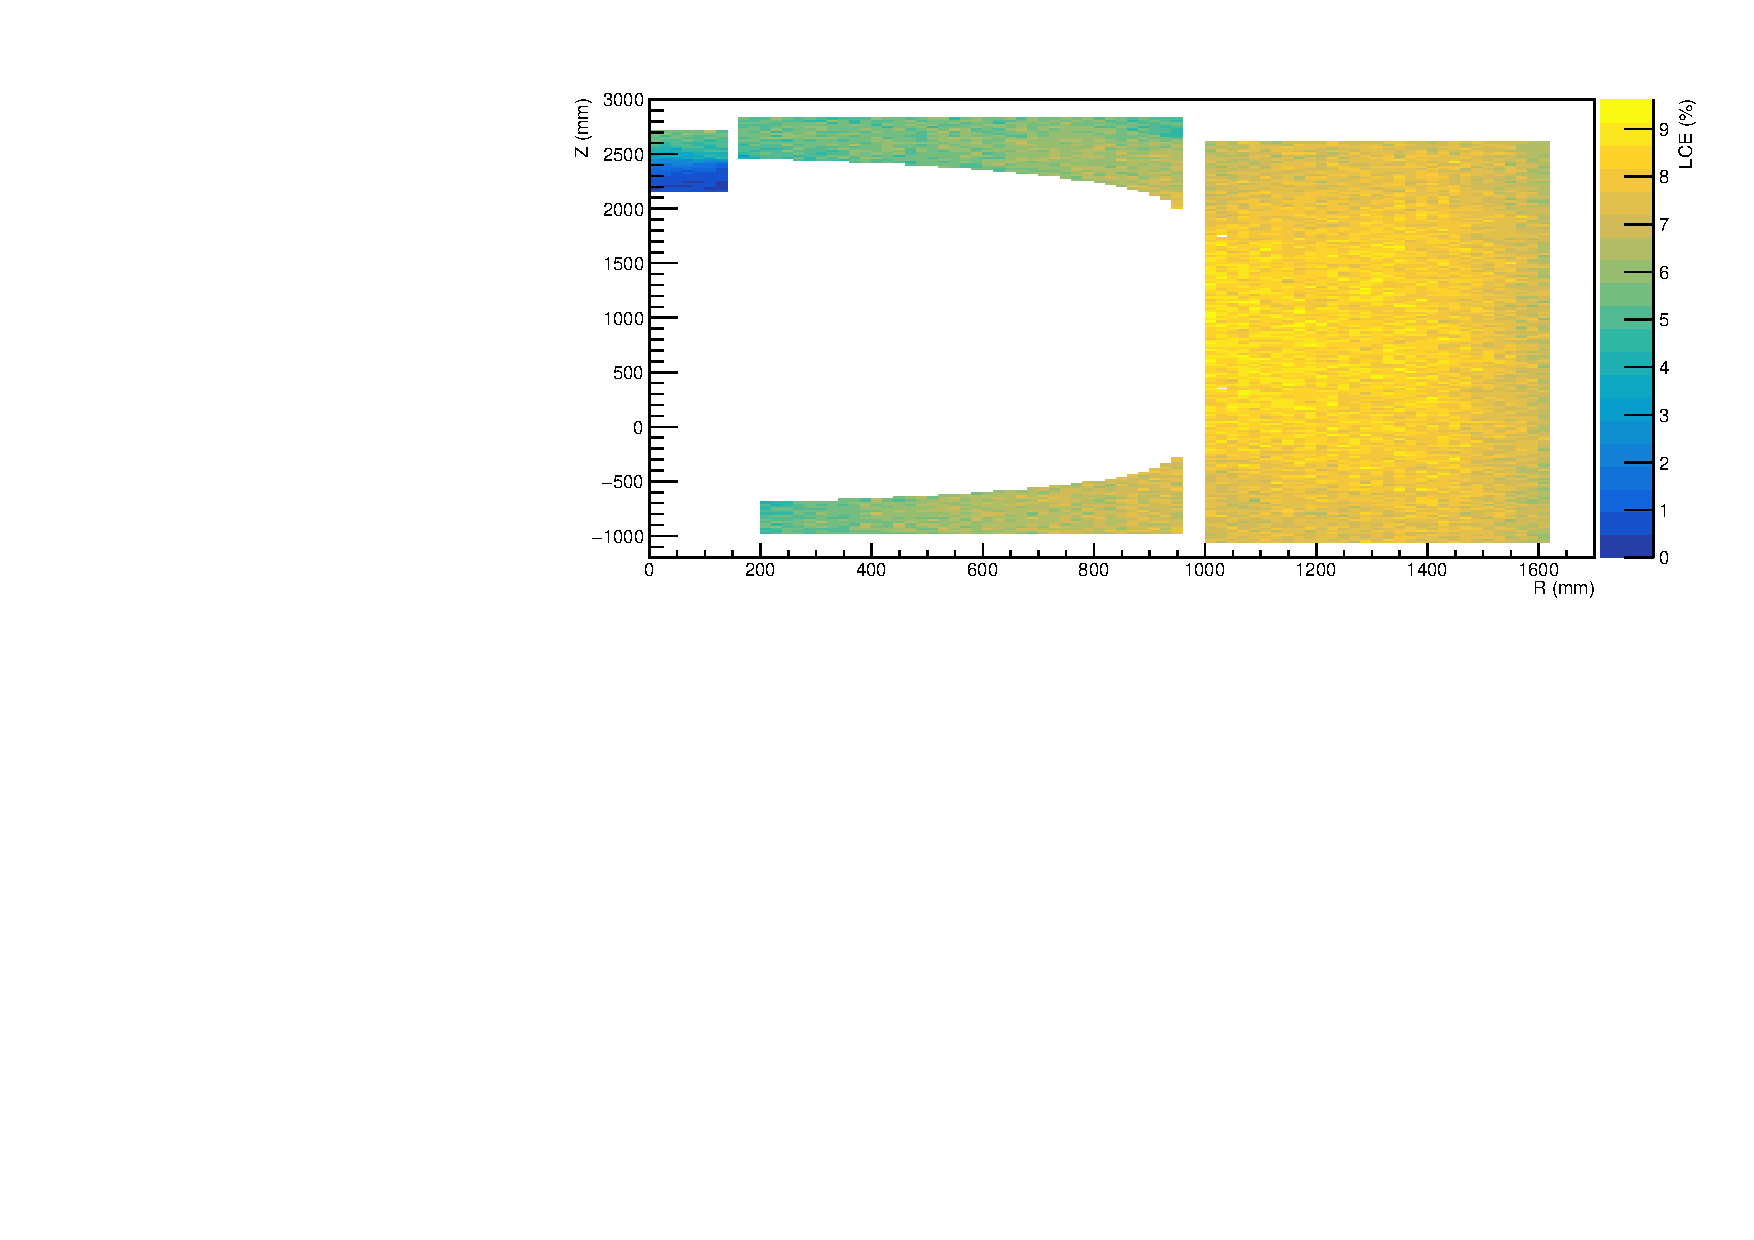
\includegraphics[width=\textwidth]{Data/GdLS_Physics/Light_Collection/od_tanks_lce.pdf}
\caption{Light Collection Efficiency for 420nm photons}
\label{fig:od_lce}
\end{figure}